\documentclass[]{article}
\usepackage{lmodern}
\usepackage{amssymb,amsmath}
\usepackage{ifxetex,ifluatex}
\usepackage{fixltx2e} % provides \textsubscript
\ifnum 0\ifxetex 1\fi\ifluatex 1\fi=0 % if pdftex
  \usepackage[T1]{fontenc}
  \usepackage[utf8]{inputenc}
\else % if luatex or xelatex
  \ifxetex
    \usepackage{mathspec}
  \else
    \usepackage{fontspec}
  \fi
  \defaultfontfeatures{Ligatures=TeX,Scale=MatchLowercase}
\fi
% use upquote if available, for straight quotes in verbatim environments
\IfFileExists{upquote.sty}{\usepackage{upquote}}{}
% use microtype if available
\IfFileExists{microtype.sty}{%
\usepackage[]{microtype}
\UseMicrotypeSet[protrusion]{basicmath} % disable protrusion for tt fonts
}{}
\PassOptionsToPackage{hyphens}{url} % url is loaded by hyperref
\usepackage[unicode=true]{hyperref}
\hypersetup{
            pdfborder={0 0 0},
            breaklinks=true}
\urlstyle{same}  % don't use monospace font for urls
\usepackage{graphicx,grffile}
\makeatletter
\def\maxwidth{\ifdim\Gin@nat@width>\linewidth\linewidth\else\Gin@nat@width\fi}
\def\maxheight{\ifdim\Gin@nat@height>\textheight\textheight\else\Gin@nat@height\fi}
\makeatother
% Scale images if necessary, so that they will not overflow the page
% margins by default, and it is still possible to overwrite the defaults
% using explicit options in \includegraphics[width, height, ...]{}
\setkeys{Gin}{width=\maxwidth,height=\maxheight,keepaspectratio}
\IfFileExists{parskip.sty}{%
\usepackage{parskip}
}{% else
\setlength{\parindent}{0pt}
\setlength{\parskip}{6pt plus 2pt minus 1pt}
}
\setlength{\emergencystretch}{3em}  % prevent overfull lines
\providecommand{\tightlist}{%
  \setlength{\itemsep}{0pt}\setlength{\parskip}{0pt}}
\setcounter{secnumdepth}{0}
% Redefines (sub)paragraphs to behave more like sections
\ifx\paragraph\undefined\else
\let\oldparagraph\paragraph
\renewcommand{\paragraph}[1]{\oldparagraph{#1}\mbox{}}
\fi
\ifx\subparagraph\undefined\else
\let\oldsubparagraph\subparagraph
\renewcommand{\subparagraph}[1]{\oldsubparagraph{#1}\mbox{}}
\fi

% set default figure placement to htbp
\makeatletter
\def\fps@figure{htbp}
\makeatother


\date{}

\begin{document}

\begin{quote}
\textbf{Работа 3.4.1}

Диа- и парамагнетики

\textbf{Цель работы:} измерение магнитной восприимчивости диа- и
пара­магнитного образцов.

\textbf{В работе используются:} электромагнит, аналитические весы,
милливеберметр, регулируемый источник постоянного тока, образцы.

Магнитная восприимчивость тел может быть определена методом измерения
сил, которые действуют на тела в магнитном поле. Суще­ствуют два
классических метода таких измерений: \emph{метод Фарадея} и \emph{метод
Гюи.} В методе Фарадея исследуемые образцы, имеющие форму маленьких
шариков, помещаются в область сильно неоднородного маг­нитного поля и
измеряется сила, действующая на образец. При этом для расчёта магнитной
восприимчивости необходимо знать величину градиента магнитного поля в
месте расположения образца. В методе Гюи используется тонкий и длинный
стержень, один из концов которо­го помещают в зазор электромагнита
(обычно в область однородного поля), а другой конец --- вне зазора, где
величиной магнитного поля можно пренебречь. Закон изменения поля --- от
максимального до ну­левого --- в этом случае несущественен. Найдём
выражение для магнитной силы, действующий на такой образец (рис.1).
Пусть площадь образца равна s, его магнитная проницаемость µ, а поле в
зазоре равно B. Воспользуемся для расчёта энергетическими соображениями.
Магнитная сила может быть вычислена как производная от магнитной энергии
по перемещению. Из теории известно (см.{[}1{]}), что эту производную
надо брать со знаком минус, когда постоянен поток (например, постоянный
магнит), или со знаком плюс при постоянном токе.
\end{quote}

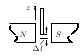
\includegraphics{./media/image1.png}

Рис. 1.Расположение

образца в зазоре

электромагнита.

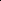
\includegraphics{./media/image2.jpeg}


\includegraphics{./media/image3.jpeg}

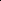
\includegraphics{./media/image2.jpeg}


\includegraphics{./media/image4.jpeg}


\includegraphics{./media/image5.jpeg}Найдём выражение для магнитной
силы, дей­ствующей на такой образец (рис. 1). Пусть пло­щадь образца
равна s, его магнитная проницае­мость --- µ, а поле в зазоре равно
\emph{В.}


\includegraphics{./media/image6.jpeg}

\begin{quote}

\includegraphics{./media/image7.jpeg}При смещении образца на расстояние
Δ\emph{l} вниз магнитная сила, дей­ствующая на него, равна

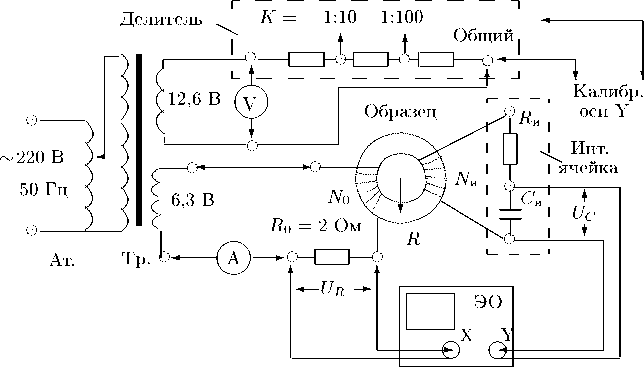
\includegraphics{./media/image8.wmf}

где \emph{ΔW\textsubscript{m} ---} изменение магнитной энергии системы
при постоянном токе в обмотке электромагнита и, следовательно, при
постоянной величине магнитного поля в зазоре.

Магнитная энергия рассчитывается по формуле

\includegraphics{./media/image9.wmf}

где интеграл распространён на всё пространство. При смещении образ­ца
магнитная энергия меняется только в области зазора (в объёме пло­щади
\emph{s} и высоты Д/), а около верхнего конца стержня остаётся
неизмен­ной, поскольку магнитного поля там практически нет. Принимая
поле внутри стержня равным измеренному нами полю в зазоре В, получим

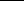
\includegraphics{./media/image10.jpeg}

\includegraphics{./media/image11.wmf}\\
Следовательно, на образец действует сила

\includegraphics{./media/image12.wmf}
\end{quote}

Знак силы, действующей на образец, зависит от знака χ: образцы из
па­рамагнитных материалов (χ \textgreater{} 0) втягиваются в зазор
электромагнита, а диамагнитные образцы (χ \textless{} 0) выталкиваются
из него.

Пренебрегая отличием \emph{µ} от единицы, получаем окончательно
рас­чётную формулу в виде

\begin{quote}
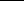
\includegraphics{./media/image13.png}

\includegraphics{./media/image14.wmf}
\end{quote}

Cледует отметить, что здесь нужно было бы учесть отличие поля в образце
от поля в зазоре, хотя в нашем случае пренебрежимо мало. В приложении
приведено решение этой задачи

.Измерив силу, действующую на образец в магнитном поле В, можно
рассчитать магнитную восприимчивость образца.

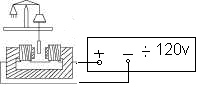
\includegraphics{./media/image15.png}

Рис. 2. Схема экспериментальной установки

\textbf{Экспериментальная установка.} Схема установки изображена на рис.
2. Магнитное поле с максимальной индукцией \textasciitilde{}1,5 Тл
создаётся в зазоре электромагнита, питаемого постоянным током. Диаметр
полю­сов существенно превосходит ширину зазора, поэтому поле в средней
части зазора достаточно однородно. Величина тока, проходящего через
обмотки электромагнита, задаётся регулируемым источником постоянного
напряжения с цифровым амперметром.

Градуировка электромагнита (связь между индукцией магнитного поля
\emph{В} в зазоре электромагнита и силой тока I в его обмотках)
про­изводится при помощи милливеберметра (описание милливеберметра и
правила работы с ним приведены на с. 148).

\begin{quote}
При измерениях образцы поочерёдно подвешиваются к аналитиче­ским весам
так, что один конец образца оказывается в зазоре электро­магнита, а
другой --- вне зазора, где индукцией магнитного поля можно

пренебречь. При помощи аналитических весов определяется перегруз­ка
\emph{ΔР = F ---} сила, действующая на образец со стороны магнитного
поля.

Как уже отмечалось, силы, действующие на диа- и парамагнитные образцы,
очень малы. Небольшие примеси ферромагнетиков (сотые до­ли процента
железа или никеля) способны кардинально изменить ре­зультат опыта,
поэтому образцы были специально отобраны. Ток через электромагнит нужно
менять только при арретированных весах,так как образцы имеют хорошую
проводимость, и токи Фуко мешают измерениям.

ЗАДАНИЕ

В работе предлагается исследовать зависимость силы, действующей на
образец, размещённый в зазоре электромагнита, от величины поля в зазоре
и по результатам измерений рассчитать магнитную восприим­чивость меди и
алюминия.
\end{quote}

\begin{enumerate}
\def\labelenumi{\arabic{enumi}.}
\item
  \begin{quote}
  Проверьте работу цепи питания электромагнита. Оцените диапазон\\
  изменения тока I через обмотки.
  \end{quote}
\item
  \begin{quote}
  Прокалибруйте электромагнит. Для этого с помощью милливебермет-\\
  ра снимите зависимость магнитного потока Ф, пронизывающего проб­\\
  ную катушку, находящуюся в зазоре, от тока \emph{I (Ф = BSN).}
  Значение\\
  \emph{SN} (произведение площади сечения пробной катушки на число
  витков\\
  в ней) указано на установке.
  \end{quote}
\end{enumerate}

\begin{quote}
\textbf{Включать и отключать электромагнит следует только при
минимальном токе.}

3. Убедитесь, что весы арретированы\textsuperscript{1}.

\textbf{Весы следует арретировать перед каждым изменением тока.}

4. Измерьте силы, действующие на образец в магнитном поле. Для это­\\
го, не включая электромагнит, подвесьте к весам один из образцов.\\
Установите на весах примерное значение массы образца (масса, диа­\\
метр и максимальное значение перегрузки для каждого образца ука­заны на
установке). Освободите весы и добейтесь точного равновесия весов.
\end{quote}

Арретируйте весы. Установите минимальное значение тока и прове­дите
измерение равновесного значения массы.

\begin{quote}
Повторите измерения m = \emph{f(I)} для 6-8 других значений тока.
\end{quote}


\includegraphics{./media/image16.jpeg}

\textsuperscript{1} Арретир (фр. arreter --- фиксировать) ---
приспособление для закрепления чув­ствительного элемента измерительного
прибора в нерабочем состоянии.

\begin{quote}
5. Повторите измерения п. 4 для другого образца.
\end{quote}

Обработка результатов

\begin{enumerate}
\def\labelenumi{\arabic{enumi}.}
\item
  Рассчитайте поле \emph{В} и постройте градуировочную кривую для
  элек­\\
  тромагнита: \emph{В =(I}).
\item
  Постройте на одном листе графики \textbar{}ΔР\textbar{} = \emph{f(B)}
  для меди и алюми­-\\
  ния.
\item
  По наклонам полученных прямых рассчитайте величину \emph{χ с} помо-­\\
  щью формулы (4).
\item
  Оцените погрешности измерений и сравните результаты с табличны-­\\
  ми значениями.
\end{enumerate}

\begin{quote}
\textbf{Контрольные вопросы}
\end{quote}

\begin{enumerate}
\def\labelenumi{\arabic{enumi}.}
\item
  Объясните суть метода измерения магнитной восприимчивости.
\item
  Напишите выражения для магнитной силы, действующей на образец, по-­\\
  мещённый в неоднородное магнитное поле.
\item
  Как можно убедиться в однородности или неоднородности магнитного
  поля\\
  в зазоре электромагнита?
\item
  Как проверить экспериментально, влияет ли намагниченность весов на
  ре­-\\
  зультаты измерения магнитной восприимчивости?
\item
  Пусть у вас используется образец в виде тонкой и длинной полосы,
  находящейся между полосами магнита. В первом случае плоскость образца
  перпендикулярна линиям магнитной индукции, во втором -- параллельна.
  Будет ли действующая на образец сила отличаться в этих двух случаях?
\end{enumerate}

\begin{quote}
СПИСОК ЛИТЕРАТУРЫ
\end{quote}

\begin{enumerate}
\def\labelenumi{\arabic{enumi}.}
\item
  \emph{Сивухин Д-В.} Общий курс физики. Т. III. Электричество. --- М.:
  Наука,\\
  1983. §§ 61, 75-77.
\item
  \emph{Калашников С.Г.} Электричество. --- М.: Наука, 1977. Гл. XI, §§
  109, 117,\\
  118.
\item
  \emph{Кингсеп А.С, Локшин Г.Р., Ольхов О.А.} Основы Физики. Т. 1.
  Механика,\\
  электричество и магнетизм, колебания и волны, волновая оптика. --- М.:
  Физ-\\
  матлит, 2001. Ч. II, гл. 5, § 5.2.
\end{enumerate}

\end{document}
